
% Default to the notebook output style

    


% Inherit from the specified cell style.




    
\documentclass[11pt]{article}

    
    
    \usepackage[T1]{fontenc}
    % Nicer default font (+ math font) than Computer Modern for most use cases
    \usepackage{mathpazo}

    % Basic figure setup, for now with no caption control since it's done
    % automatically by Pandoc (which extracts ![](path) syntax from Markdown).
    \usepackage{graphicx}
    % We will generate all images so they have a width \maxwidth. This means
    % that they will get their normal width if they fit onto the page, but
    % are scaled down if they would overflow the margins.
    % \makeatletter
    % \def\maxwidth{\ifdim\Gin@nat@width>\linewidth\linewidth
    % \else\Gin@nat@width\fi}
    % \makeatother
    % \let\Oldincludegraphics\includegraphics
    % % Set max figure width to be 80% of text width, for now hardcoded.
    % \renewcommand{\includegraphics}[1]{\Oldincludegraphics[width=.8\maxwidth]{#1}}
    % % Ensure that by default, figures have no caption (until we provide a
    % % proper Figure object with a Caption API and a way to capture that
    % % in the conversion process - todo).
    % \usepackage{caption}
    % \DeclareCaptionLabelFormat{nolabel}{}
    % \captionsetup{labelformat=nolabel}

    \usepackage{adjustbox} % Used to constrain images to a maximum size 
    \usepackage{xcolor} % Allow colors to be defined
    \usepackage{enumerate} % Needed for markdown enumerations to work
    \usepackage{geometry} % Used to adjust the document margins
    \usepackage{amsmath} % Equations
    \usepackage{amssymb} % Equations
    \usepackage{textcomp} % defines textquotesingle
    % Hack from http://tex.stackexchange.com/a/47451/13684:
    \AtBeginDocument{%
        \def\PYZsq{\textquotesingle}% Upright quotes in Pygmentized code
    }
    \usepackage{upquote} % Upright quotes for verbatim code
    \usepackage{eurosym} % defines \euro
    \usepackage[mathletters]{ucs} % Extended unicode (utf-8) support
    \usepackage[utf8x]{inputenc} % Allow utf-8 characters in the tex document
    \usepackage{fancyvrb} % verbatim replacement that allows latex
    \usepackage{grffile} % extends the file name processing of package graphics 
                         % to support a larger range 
    % The hyperref package gives us a pdf with properly built
    % internal navigation ('pdf bookmarks' for the table of contents,
    % internal cross-reference links, web links for URLs, etc.)
    \usepackage{hyperref}
    \usepackage{longtable} % longtable support required by pandoc >1.10
    \usepackage{booktabs}  % table support for pandoc > 1.12.2
    \usepackage[inline]{enumitem} % IRkernel/repr support (it uses the enumerate* environment)
    \usepackage[normalem]{ulem} % ulem is needed to support strikethroughs (\sout)
                                % normalem makes italics be italics, not underlines
    \usepackage{mathrsfs}
    \usepackage{float}
    \usepackage{biblatex}
    \usepackage[english]{babel}
    \addbibresource{resources.bib}
    
    % \bibliographystyle{annotate}
    % \bibliography{resources.bib}
    
    
    % Colors for the hyperref package
    \definecolor{urlcolor}{rgb}{0,.145,.698}
    \definecolor{linkcolor}{rgb}{.71,0.21,0.01}
    \definecolor{citecolor}{rgb}{.12,.54,.11}

    % ANSI colors
    \definecolor{ansi-black}{HTML}{3E424D}
    \definecolor{ansi-black-intense}{HTML}{282C36}
    \definecolor{ansi-red}{HTML}{E75C58}
    \definecolor{ansi-red-intense}{HTML}{B22B31}
    \definecolor{ansi-green}{HTML}{00A250}
    \definecolor{ansi-green-intense}{HTML}{007427}
    \definecolor{ansi-yellow}{HTML}{DDB62B}
    \definecolor{ansi-yellow-intense}{HTML}{B27D12}
    \definecolor{ansi-blue}{HTML}{208FFB}
    \definecolor{ansi-blue-intense}{HTML}{0065CA}
    \definecolor{ansi-magenta}{HTML}{D160C4}
    \definecolor{ansi-magenta-intense}{HTML}{A03196}
    \definecolor{ansi-cyan}{HTML}{60C6C8}
    \definecolor{ansi-cyan-intense}{HTML}{258F8F}
    \definecolor{ansi-white}{HTML}{C5C1B4}
    \definecolor{ansi-white-intense}{HTML}{A1A6B2}
    \definecolor{ansi-default-inverse-fg}{HTML}{FFFFFF}
    \definecolor{ansi-default-inverse-bg}{HTML}{000000}

    % commands and environments needed by pandoc snippets
    % extracted from the output of `pandoc -s`
    \providecommand{\tightlist}{%
      \setlength{\itemsep}{0pt}\setlength{\parskip}{0pt}}
    \DefineVerbatimEnvironment{Highlighting}{Verbatim}{commandchars=\\\{\}}
    % Add ',fontsize=\small' for more characters per line
    \newenvironment{Shaded}{}{}
    \newcommand{\KeywordTok}[1]{\textcolor[rgb]{0.00,0.44,0.13}{\textbf{{#1}}}}
    \newcommand{\DataTypeTok}[1]{\textcolor[rgb]{0.56,0.13,0.00}{{#1}}}
    \newcommand{\DecValTok}[1]{\textcolor[rgb]{0.25,0.63,0.44}{{#1}}}
    \newcommand{\BaseNTok}[1]{\textcolor[rgb]{0.25,0.63,0.44}{{#1}}}
    \newcommand{\FloatTok}[1]{\textcolor[rgb]{0.25,0.63,0.44}{{#1}}}
    \newcommand{\CharTok}[1]{\textcolor[rgb]{0.25,0.44,0.63}{{#1}}}
    \newcommand{\StringTok}[1]{\textcolor[rgb]{0.25,0.44,0.63}{{#1}}}
    \newcommand{\CommentTok}[1]{\textcolor[rgb]{0.38,0.63,0.69}{\textit{{#1}}}}
    \newcommand{\OtherTok}[1]{\textcolor[rgb]{0.00,0.44,0.13}{{#1}}}
    \newcommand{\AlertTok}[1]{\textcolor[rgb]{1.00,0.00,0.00}{\textbf{{#1}}}}
    \newcommand{\FunctionTok}[1]{\textcolor[rgb]{0.02,0.16,0.49}{{#1}}}
    \newcommand{\RegionMarkerTok}[1]{{#1}}
    \newcommand{\ErrorTok}[1]{\textcolor[rgb]{1.00,0.00,0.00}{\textbf{{#1}}}}
    \newcommand{\NormalTok}[1]{{#1}}
    
    % Additional commands for more recent versions of Pandoc
    \newcommand{\ConstantTok}[1]{\textcolor[rgb]{0.53,0.00,0.00}{{#1}}}
    \newcommand{\SpecialCharTok}[1]{\textcolor[rgb]{0.25,0.44,0.63}{{#1}}}
    \newcommand{\VerbatimStringTok}[1]{\textcolor[rgb]{0.25,0.44,0.63}{{#1}}}
    \newcommand{\SpecialStringTok}[1]{\textcolor[rgb]{0.73,0.40,0.53}{{#1}}}
    \newcommand{\ImportTok}[1]{{#1}}
    \newcommand{\DocumentationTok}[1]{\textcolor[rgb]{0.73,0.13,0.13}{\textit{{#1}}}}
    \newcommand{\AnnotationTok}[1]{\textcolor[rgb]{0.38,0.63,0.69}{\textbf{\textit{{#1}}}}}
    \newcommand{\CommentVarTok}[1]{\textcolor[rgb]{0.38,0.63,0.69}{\textbf{\textit{{#1}}}}}
    \newcommand{\VariableTok}[1]{\textcolor[rgb]{0.10,0.09,0.49}{{#1}}}
    \newcommand{\ControlFlowTok}[1]{\textcolor[rgb]{0.00,0.44,0.13}{\textbf{{#1}}}}
    \newcommand{\OperatorTok}[1]{\textcolor[rgb]{0.40,0.40,0.40}{{#1}}}
    \newcommand{\BuiltInTok}[1]{{#1}}
    \newcommand{\ExtensionTok}[1]{{#1}}
    \newcommand{\PreprocessorTok}[1]{\textcolor[rgb]{0.74,0.48,0.00}{{#1}}}
    \newcommand{\AttributeTok}[1]{\textcolor[rgb]{0.49,0.56,0.16}{{#1}}}
    \newcommand{\InformationTok}[1]{\textcolor[rgb]{0.38,0.63,0.69}{\textbf{\textit{{#1}}}}}
    \newcommand{\WarningTok}[1]{\textcolor[rgb]{0.38,0.63,0.69}{\textbf{\textit{{#1}}}}}
    
    
    % Define a nice break command that doesn't care if a line doesn't already
    % exist.
    \def\br{\hspace*{\fill} \\* }
    % Math Jax compatibility definitions
    \def\gt{>}
    \def\lt{<}
    \let\Oldtex\TeX
    \let\Oldlatex\LaTeX
    \renewcommand{\TeX}{\textrm{\Oldtex}}
    \renewcommand{\LaTeX}{\textrm{\Oldlatex}}
    % Document parameters
    % Document title
    \title{Ensemble Classification as an Effective Method of Determining Racial Bias in Incarceration Data}
    
    \date{April 15, 2020}
    
    
    

    % Pygments definitions
    
\makeatletter
\def\PY@reset{\let\PY@it=\relax \let\PY@bf=\relax%
    \let\PY@ul=\relax \let\PY@tc=\relax%
    \let\PY@bc=\relax \let\PY@ff=\relax}
\def\PY@tok#1{\csname PY@tok@#1\endcsname}
\def\PY@toks#1+{\ifx\relax#1\empty\else%
    \PY@tok{#1}\expandafter\PY@toks\fi}
\def\PY@do#1{\PY@bc{\PY@tc{\PY@ul{%
    \PY@it{\PY@bf{\PY@ff{#1}}}}}}}
\def\PY#1#2{\PY@reset\PY@toks#1+\relax+\PY@do{#2}}

\expandafter\def\csname PY@tok@w\endcsname{\def\PY@tc##1{\textcolor[rgb]{0.73,0.73,0.73}{##1}}}
\expandafter\def\csname PY@tok@c\endcsname{\let\PY@it=\textit\def\PY@tc##1{\textcolor[rgb]{0.25,0.50,0.50}{##1}}}
\expandafter\def\csname PY@tok@cp\endcsname{\def\PY@tc##1{\textcolor[rgb]{0.74,0.48,0.00}{##1}}}
\expandafter\def\csname PY@tok@k\endcsname{\let\PY@bf=\textbf\def\PY@tc##1{\textcolor[rgb]{0.00,0.50,0.00}{##1}}}
\expandafter\def\csname PY@tok@kp\endcsname{\def\PY@tc##1{\textcolor[rgb]{0.00,0.50,0.00}{##1}}}
\expandafter\def\csname PY@tok@kt\endcsname{\def\PY@tc##1{\textcolor[rgb]{0.69,0.00,0.25}{##1}}}
\expandafter\def\csname PY@tok@o\endcsname{\def\PY@tc##1{\textcolor[rgb]{0.40,0.40,0.40}{##1}}}
\expandafter\def\csname PY@tok@ow\endcsname{\let\PY@bf=\textbf\def\PY@tc##1{\textcolor[rgb]{0.67,0.13,1.00}{##1}}}
\expandafter\def\csname PY@tok@nb\endcsname{\def\PY@tc##1{\textcolor[rgb]{0.00,0.50,0.00}{##1}}}
\expandafter\def\csname PY@tok@nf\endcsname{\def\PY@tc##1{\textcolor[rgb]{0.00,0.00,1.00}{##1}}}
\expandafter\def\csname PY@tok@nc\endcsname{\let\PY@bf=\textbf\def\PY@tc##1{\textcolor[rgb]{0.00,0.00,1.00}{##1}}}
\expandafter\def\csname PY@tok@nn\endcsname{\let\PY@bf=\textbf\def\PY@tc##1{\textcolor[rgb]{0.00,0.00,1.00}{##1}}}
\expandafter\def\csname PY@tok@ne\endcsname{\let\PY@bf=\textbf\def\PY@tc##1{\textcolor[rgb]{0.82,0.25,0.23}{##1}}}
\expandafter\def\csname PY@tok@nv\endcsname{\def\PY@tc##1{\textcolor[rgb]{0.10,0.09,0.49}{##1}}}
\expandafter\def\csname PY@tok@no\endcsname{\def\PY@tc##1{\textcolor[rgb]{0.53,0.00,0.00}{##1}}}
\expandafter\def\csname PY@tok@nl\endcsname{\def\PY@tc##1{\textcolor[rgb]{0.63,0.63,0.00}{##1}}}
\expandafter\def\csname PY@tok@ni\endcsname{\let\PY@bf=\textbf\def\PY@tc##1{\textcolor[rgb]{0.60,0.60,0.60}{##1}}}
\expandafter\def\csname PY@tok@na\endcsname{\def\PY@tc##1{\textcolor[rgb]{0.49,0.56,0.16}{##1}}}
\expandafter\def\csname PY@tok@nt\endcsname{\let\PY@bf=\textbf\def\PY@tc##1{\textcolor[rgb]{0.00,0.50,0.00}{##1}}}
\expandafter\def\csname PY@tok@nd\endcsname{\def\PY@tc##1{\textcolor[rgb]{0.67,0.13,1.00}{##1}}}
\expandafter\def\csname PY@tok@s\endcsname{\def\PY@tc##1{\textcolor[rgb]{0.73,0.13,0.13}{##1}}}
\expandafter\def\csname PY@tok@sd\endcsname{\let\PY@it=\textit\def\PY@tc##1{\textcolor[rgb]{0.73,0.13,0.13}{##1}}}
\expandafter\def\csname PY@tok@si\endcsname{\let\PY@bf=\textbf\def\PY@tc##1{\textcolor[rgb]{0.73,0.40,0.53}{##1}}}
\expandafter\def\csname PY@tok@se\endcsname{\let\PY@bf=\textbf\def\PY@tc##1{\textcolor[rgb]{0.73,0.40,0.13}{##1}}}
\expandafter\def\csname PY@tok@sr\endcsname{\def\PY@tc##1{\textcolor[rgb]{0.73,0.40,0.53}{##1}}}
\expandafter\def\csname PY@tok@ss\endcsname{\def\PY@tc##1{\textcolor[rgb]{0.10,0.09,0.49}{##1}}}
\expandafter\def\csname PY@tok@sx\endcsname{\def\PY@tc##1{\textcolor[rgb]{0.00,0.50,0.00}{##1}}}
\expandafter\def\csname PY@tok@m\endcsname{\def\PY@tc##1{\textcolor[rgb]{0.40,0.40,0.40}{##1}}}
\expandafter\def\csname PY@tok@gh\endcsname{\let\PY@bf=\textbf\def\PY@tc##1{\textcolor[rgb]{0.00,0.00,0.50}{##1}}}
\expandafter\def\csname PY@tok@gu\endcsname{\let\PY@bf=\textbf\def\PY@tc##1{\textcolor[rgb]{0.50,0.00,0.50}{##1}}}
\expandafter\def\csname PY@tok@gd\endcsname{\def\PY@tc##1{\textcolor[rgb]{0.63,0.00,0.00}{##1}}}
\expandafter\def\csname PY@tok@gi\endcsname{\def\PY@tc##1{\textcolor[rgb]{0.00,0.63,0.00}{##1}}}
\expandafter\def\csname PY@tok@gr\endcsname{\def\PY@tc##1{\textcolor[rgb]{1.00,0.00,0.00}{##1}}}
\expandafter\def\csname PY@tok@ge\endcsname{\let\PY@it=\textit}
\expandafter\def\csname PY@tok@gs\endcsname{\let\PY@bf=\textbf}
\expandafter\def\csname PY@tok@gp\endcsname{\let\PY@bf=\textbf\def\PY@tc##1{\textcolor[rgb]{0.00,0.00,0.50}{##1}}}
\expandafter\def\csname PY@tok@go\endcsname{\def\PY@tc##1{\textcolor[rgb]{0.53,0.53,0.53}{##1}}}
\expandafter\def\csname PY@tok@gt\endcsname{\def\PY@tc##1{\textcolor[rgb]{0.00,0.27,0.87}{##1}}}
\expandafter\def\csname PY@tok@err\endcsname{\def\PY@bc##1{\setlength{\fboxsep}{0pt}\fcolorbox[rgb]{1.00,0.00,0.00}{1,1,1}{\strut ##1}}}
\expandafter\def\csname PY@tok@kc\endcsname{\let\PY@bf=\textbf\def\PY@tc##1{\textcolor[rgb]{0.00,0.50,0.00}{##1}}}
\expandafter\def\csname PY@tok@kd\endcsname{\let\PY@bf=\textbf\def\PY@tc##1{\textcolor[rgb]{0.00,0.50,0.00}{##1}}}
\expandafter\def\csname PY@tok@kn\endcsname{\let\PY@bf=\textbf\def\PY@tc##1{\textcolor[rgb]{0.00,0.50,0.00}{##1}}}
\expandafter\def\csname PY@tok@kr\endcsname{\let\PY@bf=\textbf\def\PY@tc##1{\textcolor[rgb]{0.00,0.50,0.00}{##1}}}
\expandafter\def\csname PY@tok@bp\endcsname{\def\PY@tc##1{\textcolor[rgb]{0.00,0.50,0.00}{##1}}}
\expandafter\def\csname PY@tok@fm\endcsname{\def\PY@tc##1{\textcolor[rgb]{0.00,0.00,1.00}{##1}}}
\expandafter\def\csname PY@tok@vc\endcsname{\def\PY@tc##1{\textcolor[rgb]{0.10,0.09,0.49}{##1}}}
\expandafter\def\csname PY@tok@vg\endcsname{\def\PY@tc##1{\textcolor[rgb]{0.10,0.09,0.49}{##1}}}
\expandafter\def\csname PY@tok@vi\endcsname{\def\PY@tc##1{\textcolor[rgb]{0.10,0.09,0.49}{##1}}}
\expandafter\def\csname PY@tok@vm\endcsname{\def\PY@tc##1{\textcolor[rgb]{0.10,0.09,0.49}{##1}}}
\expandafter\def\csname PY@tok@sa\endcsname{\def\PY@tc##1{\textcolor[rgb]{0.73,0.13,0.13}{##1}}}
\expandafter\def\csname PY@tok@sb\endcsname{\def\PY@tc##1{\textcolor[rgb]{0.73,0.13,0.13}{##1}}}
\expandafter\def\csname PY@tok@sc\endcsname{\def\PY@tc##1{\textcolor[rgb]{0.73,0.13,0.13}{##1}}}
\expandafter\def\csname PY@tok@dl\endcsname{\def\PY@tc##1{\textcolor[rgb]{0.73,0.13,0.13}{##1}}}
\expandafter\def\csname PY@tok@s2\endcsname{\def\PY@tc##1{\textcolor[rgb]{0.73,0.13,0.13}{##1}}}
\expandafter\def\csname PY@tok@sh\endcsname{\def\PY@tc##1{\textcolor[rgb]{0.73,0.13,0.13}{##1}}}
\expandafter\def\csname PY@tok@s1\endcsname{\def\PY@tc##1{\textcolor[rgb]{0.73,0.13,0.13}{##1}}}
\expandafter\def\csname PY@tok@mb\endcsname{\def\PY@tc##1{\textcolor[rgb]{0.40,0.40,0.40}{##1}}}
\expandafter\def\csname PY@tok@mf\endcsname{\def\PY@tc##1{\textcolor[rgb]{0.40,0.40,0.40}{##1}}}
\expandafter\def\csname PY@tok@mh\endcsname{\def\PY@tc##1{\textcolor[rgb]{0.40,0.40,0.40}{##1}}}
\expandafter\def\csname PY@tok@mi\endcsname{\def\PY@tc##1{\textcolor[rgb]{0.40,0.40,0.40}{##1}}}
\expandafter\def\csname PY@tok@il\endcsname{\def\PY@tc##1{\textcolor[rgb]{0.40,0.40,0.40}{##1}}}
\expandafter\def\csname PY@tok@mo\endcsname{\def\PY@tc##1{\textcolor[rgb]{0.40,0.40,0.40}{##1}}}
\expandafter\def\csname PY@tok@ch\endcsname{\let\PY@it=\textit\def\PY@tc##1{\textcolor[rgb]{0.25,0.50,0.50}{##1}}}
\expandafter\def\csname PY@tok@cm\endcsname{\let\PY@it=\textit\def\PY@tc##1{\textcolor[rgb]{0.25,0.50,0.50}{##1}}}
\expandafter\def\csname PY@tok@cpf\endcsname{\let\PY@it=\textit\def\PY@tc##1{\textcolor[rgb]{0.25,0.50,0.50}{##1}}}
\expandafter\def\csname PY@tok@c1\endcsname{\let\PY@it=\textit\def\PY@tc##1{\textcolor[rgb]{0.25,0.50,0.50}{##1}}}
\expandafter\def\csname PY@tok@cs\endcsname{\let\PY@it=\textit\def\PY@tc##1{\textcolor[rgb]{0.25,0.50,0.50}{##1}}}

\def\PYZbs{\char`\\}
\def\PYZus{\char`\_}
\def\PYZob{\char`\{}
\def\PYZcb{\char`\}}
\def\PYZca{\char`\^}
\def\PYZam{\char`\&}
\def\PYZlt{\char`\<}
\def\PYZgt{\char`\>}
\def\PYZsh{\char`\#}
\def\PYZpc{\char`\%}
\def\PYZdl{\char`\$}
\def\PYZhy{\char`\-}
\def\PYZsq{\char`\'}
\def\PYZdq{\char`\"}
\def\PYZti{\char`\~}
% for compatibility with earlier versions
\def\PYZat{@}
\def\PYZlb{[}
\def\PYZrb{]}
\makeatother


    % Exact colors from NB
    \definecolor{incolor}{rgb}{0.0, 0.0, 0.5}
    \definecolor{outcolor}{rgb}{0.545, 0.0, 0.0}



    
    % Prevent overflowing lines due to hard-to-break entities
    \sloppy 
    % Setup hyperref package
    \hypersetup{
      breaklinks=true,  % so long urls are correctly broken across lines
      colorlinks=true,
      urlcolor=urlcolor,
      linkcolor=linkcolor,
      citecolor=citecolor,
      }
    % Slightly bigger margins than the latex defaults
    
    \geometry{verbose,tmargin=1in,bmargin=1in,lmargin=1in,rmargin=1in}
    
    

    \begin{document}
    
    
    \maketitle
    
    

   
    \hypertarget{abstract}{%
\section*{}\label{abstract}}
\begin{abstract}
Machine Learning is becoming a more prevalent tool in the world of
criminal justice. Often it is used to predict who will commit a crime or
where crimes may occur. Seldom is it used to regulate the criminal
justice system, however. In this report I examine prison inmate data
and determine what machine learning techniques are effective at
detecting the racial bias that has been shown to exist in this data. In
this report I find that ensemble methods, especially LightGBM, are effective in classifying inmates by race, thus showing that racial bias is detectable by machine learning techniques and that machine learning is an effective tool in determining if criminal justice reform should be considered. 
\end{abstract}

\hypertarget{problem-statement-and-motivation}{%
\section{Problem Statement and
Motivation}\label{problem-statement-and-motivation}}

Last semester I took a look a data set containing the information of
more than 7.5 million individuals that have been processed by the
criminal justice system. I found that racial minorities were more likely
to receive extreme sentences, agreeing with existing research around
bias in the criminal justice system\cite{me}. In this report I will be exploring
the data from a machine learning perspective. My goal is to determine if
this data can be classified in such a way that is predictive of race.
The idea is that perhaps racial bias can be detected in various systems
by seeing how effective different machine learning techniques are at
classifying an inmate's by race given their data.

This is an unconventional way to approach criminal justice data with
machine learning. Often we see machine learning being used to attempt to
determine who might be a criminal or where criminal activity may occur
using social media data and other public information, which may include
data the government owns, but which is not available to the public. These
approaches often ignore or discount the ways that these techniques may
disproportionately affect people of color and the poor. Many
organizations have made official statements regarding the use of
machine learning in this way, often called predictive policing. The
ACLU for example released a statement listing civil rights related
concerns about predictive policing which was signed by several civil
rights organizations including the NAACP\cite{aclu}.

My objective is to go against the predictive policing paradigm and use
machine learning to benefit these negatively affected classes of people
by using machine learning as a diagnostic tool. If it can be shown that
certain machine learning techniques are effective at classifying inmates
by race given incarceration related information, then we can inform
policies that will attempt to correct for these systemic racial biases.

    \hypertarget{data}{%
\section{Data}\label{data}}

\hypertarget{source-and-credibility}{%
\subsection{Source and Credibility}\label{source-and-credibility}}

The data that I will be using in this analysis is from one source. It is
a
\href{https://catalog.data.gov/dataset/sentenced-inmates-in-correctional-facilities}{database}
hosted on \href{https://www.data.gov}{Data.gov} and maintained by the
State of Connecticut Department of Corrections. This source is highly
credible because it is a primary source for the data. This organization
is an official government agency which collects, maintains, and reports
on this data.

\hypertarget{gathering-and-cleaning}{%
\subsection{Gathering and Cleaning}\label{gathering-and-cleaning}}

All the data which I am using in this report are freely available to the
public. Collection and cleaning was relatively simple as the source data
was well maintained. The file that I obtained from the Connecticut
Department of Corrections is a very well maintained database. The
largest issue I had with this file was mild inconsistency with the way
in which certain data was encoded (ex. race was encoded as both
\texttt{WHITE} and \texttt{WHITE\textbackslash{}t}). The file is

\begin{verbatim}
individuals.csv.
\end{verbatim}

\hypertarget{about-the-data}{%
\subsection{About the Data}\label{about-the-data}}

This data set contains individual information for 7.77 million people
that have been processed by the justice system and recorded by the
Connecticut Department of Corrections. Each individual is recorded along
with their age, gender, race, offense, and sentence length, among other
things.

Because there is so much to consider in what is found in the data set, I
chose not to feature engineer as to avoid unneeded complexity.

The sample sizes among different races that are found in the Connecticut
Department of Justice data are not similar. The sample size for American
Indians and Asians is much smaller than that of Whites, Hispanics, and
Blacks, hence we may see some irregular outcomes in the analysis related
to these racial groups.

    \begin{Verbatim}[commandchars=\\\{\}]
Sample size for Blacks: 3287596
Sample size for Whites: 2393949
Sample size for Hispanic: 2039297
Sample size for American Indian: 21133
Sample size for Asian: 35660

    \end{Verbatim}

    \hypertarget{methods}{%
\section{Methods}\label{methods}}

Before I begin discussing the methods that I did use, I will talk about
some of the methods that I did not use. There are many techniques that
are not applicable to this data. For example, since this data set is not
a time series models like ARMA and HMM are not applicable here.

\hypertarget{dimension-reduction}{%
\subsection{Dimension Reduction}\label{dimension-reduction}}

A method that I attempted to use, but found little success with were
dimension reduction tools like PCA, T-SNE, and UMAP. This dimension
reduction would have been helpful, especially because once one-hot
encoded this data becomes extremely high dimensional. However PCA,
T-SNE, and UMAP all failed to create meaningful clusters, so I abandoned
the the pursuit of clustering early on. Perhaps some kernel methods
would have been helpful in this endeavor, however I could not find a
kernel that could create a metric on crimes and I do not feel qualified
to write one myself.

Below I have images of my attempt to use PCA, T-SNE, and UMAP to cluster
the data. It is apparent that these methods are simply not effective.

    \begin{figure}
        \centering
        \begin{tabular}{c c}
            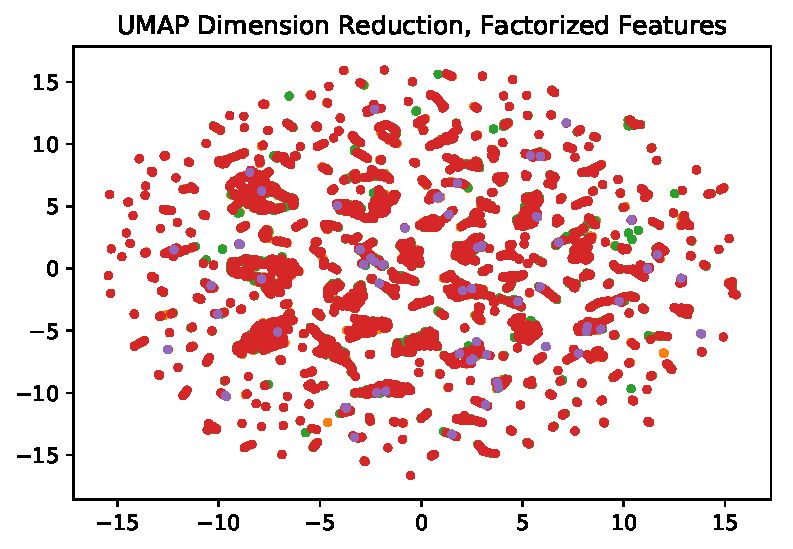
\includegraphics[scale=.5]{images/UMAP1.pdf}  & 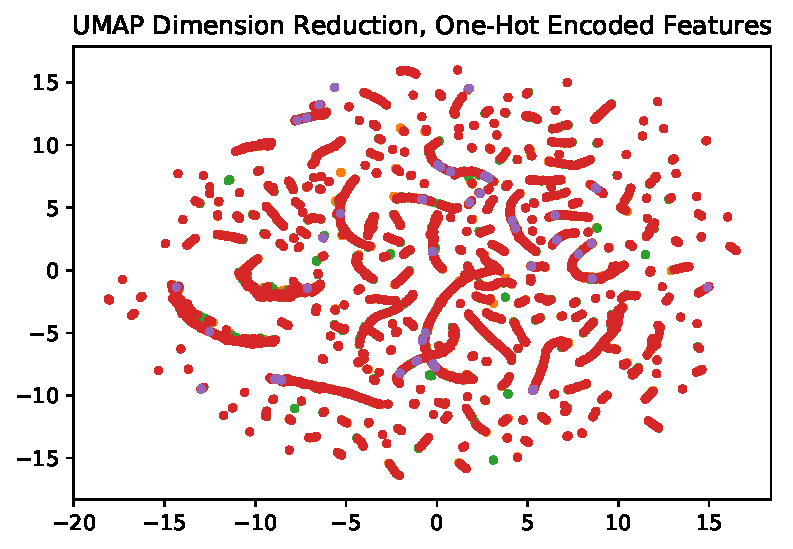
\includegraphics[scale=.5]{images/UMAP2.pdf} \\
            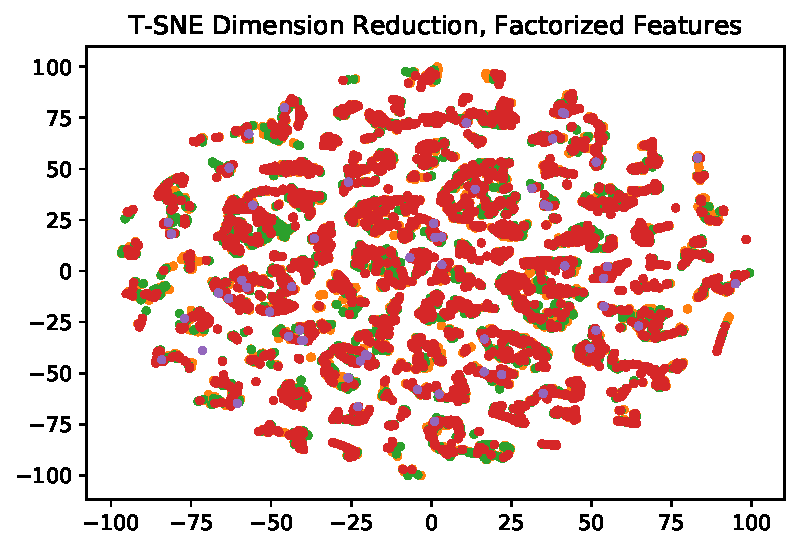
\includegraphics[scale=.5]{images/TSNE1.pdf} & 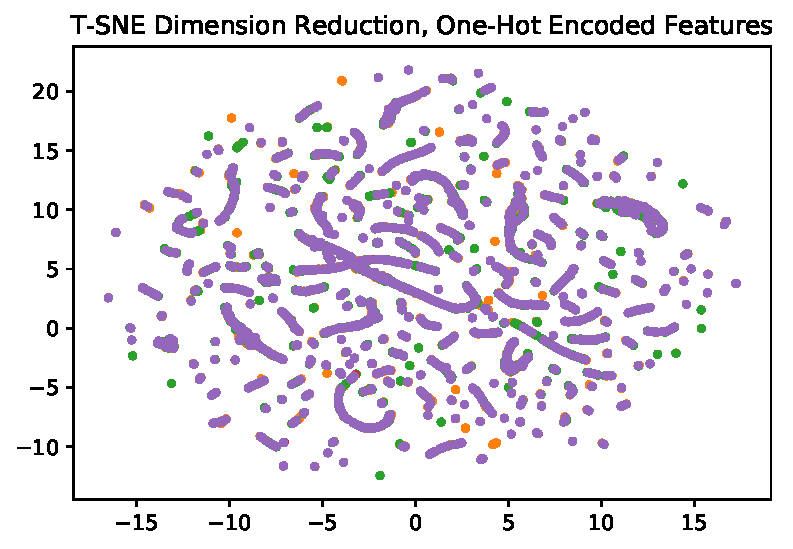
\includegraphics[scale=.5]{images/TSNE2.pdf}
        \end{tabular}
        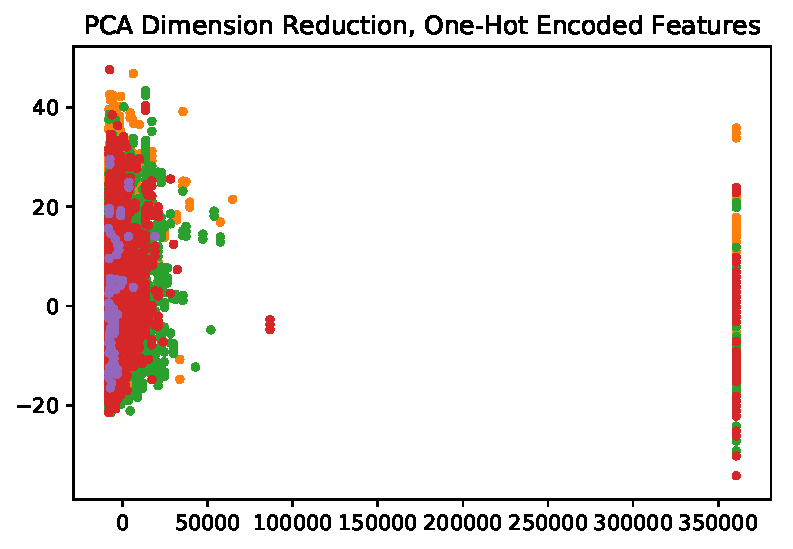
\includegraphics[scale=.5]{images/PCA.pdf}
        \caption{Dimension reduction algorithms fail to reveal significant clusters}
        \label{fig:my_label}
    \end{figure}
    { \hspace*{\fill} \\}
    
    
    This is only a small sample of things that I tried to do to get useful
clustering given the dimension reduction, though it is representative
of the results I found.

    \hypertarget{ensemble-methods}{%
\subsection{Ensemble Methods}\label{ensemble-methods}}

Ensemble methods seemed immediately like the methods with the highest chance of success. I did not initially expect to successfully classify this data, however as I learned about how ensemble classifiers worked I became more confident that I would get decent results.

The primary reason that I though I would not get good results has to do
with how I identified racial bias in the data. In my previous report I
determined that there was racial bias in the criminal justice system
based on the kurtosis of the distribution of sentence lengths, when
blocking inmates by race. Interpreted this means that minorities are much
more likely to receive extreme sentence lengths than a white people
are. This condition is very subtle and I did not think that it would be
easily detectable by machine learning methods. However, ensemble methods
only need each member to do slightly better than random, so there was
hope that I could get good results with these methods.

The methods that I attempted were the following: random forest
classifier, gradient descent boosted classifier, XGBoost, and LightGBM.

    \hypertarget{lightgbm}{%
\subsubsection{LightGBM}\label{lightgbm}}

LightGBM is an attempt to improve upon the efficiency, both temporally
and spatially, of different gradient boosted decision tree (GBDT)
algorithms such as XGBoost. This algorithm was developed by a team at
Microsoft and it uses two novel techniques to improve GBDT algorithms.
The baseline comparison used was against XGBoost, since the team found
this method to be the best performer of the commonly used GBDT
algorithms\cite{lgbm}.

By analyzing GBDT algorithms the team found that the most expensive
parts of the process is learning the decision trees and the most
expensive part of learning the decision trees is finding the best split
points. They decided to use a histogram based approach for efficiency.
This process is dominated by the histogram building which has a
complexity of $O(\#data \times \#feature)$\footnote{LightGBM is not the only GDBT classifier that uses a histogram approach to finding splitting points. XGBoost also can be programmed to use this method.}. Now the goal is to reduce
the feature number or the number of data points.

\hypertarget{gradient-based-one-side-sampling}{%
\paragraph{Gradient-based One-Side
Sampling}\label{gradient-based-one-side-sampling}}

This is the first novel technique proposed by the Microsoft team. It is
a sampling method that is meant to reduce the number of data instances
while maintaining accuracy. The main idea here is that data points with
small gradient are usually ignored, since the model is already will
trained on those data instances. However, the changes that occur by
ignoring the data will small gradient may reduce the accuracy of the
model once it is learned. Therefore GOSS examines all of the high
gradient data and a random sample of the small gradient data. This
method can maximize the amount of relevant data used in the training of
the model without handicapping the accuracy completely.

\hypertarget{exclusive-feature-bundling}{%
\paragraph{Exclusive Feature
Bundling}\label{exclusive-feature-bundling}}

This is the second novel technique and its goal is to reduce the number
of features. This technique relies on the fact that high dimensional
data tend to be sparse, and therefore there are likely large bundles of
features that are mutually exclusive are nearly mutually exclusive.
These features can be bundled into a single feature and their histograms
can be combined. This reduces the complexity of building histograms from
$O(\#data \times \#feature)$ to $O(\#data \times \#bundle)$ and if
$\#bundle << \#feature$ then the total complexity is greatly reduced.

    \hypertarget{results}{%
\section{Results}\label{results}}

\hypertarget{random-forest-classifier}{%
\subsection{Random Forest Classifier}\label{random-forest-classifier}}

The random forest classifier was an easy place to begin in my attempt to
find a successful classifier. It is a simple method and would likely
give me a good lower bound on the success that I would have.

In using the random forest classifier I did a grid-search for the best
parameters. The parameters I decided to search over are the number of
trees in the classifier and the maximum depth of the trees in the
classifier. I chose this because having more trees in the classifier
will improve the accuracy, however if the depth of each of the trees in
unbounded then overfitting of the individual trees may become an issue.

In my grid-search I found the best parameters to be the following

    \begin{Verbatim}[commandchars=\\\{\}]
Max Depth = 85
Number of Estimators = 2100.
    \end{Verbatim}

    My results with the random forest classifier were rather disappointing,
especially given the amount of time it took to train which was 5.32
hours on the following parameter grid

\begin{Shaded}
\begin{Highlighting}[]
\NormalTok{param_grid }\OperatorTok{=}\NormalTok{ \{}
    \StringTok{'n_estimators'}\NormalTok{: np.arange(}\DecValTok{100}\NormalTok{,}\DecValTok{5100}\NormalTok{,}\DecValTok{500}\NormalTok{),}
    \StringTok{'max_depth'}\NormalTok{: np.arange(}\DecValTok{5}\NormalTok{,}\DecValTok{100}\NormalTok{,}\DecValTok{10}\NormalTok{)}
\NormalTok{\}}
\end{Highlighting}
\end{Shaded}

The out-of-box score was rather promising at .70 however the method
scored barely better than chance, which is .2 given that there are 5 race classes in the data. Here is a scoring of the model I ran:

    \begin{Verbatim}[commandchars=\\\{\}]
score on a test size of 500000 is 0.286932.
    \end{Verbatim}

    The scoring here is lackluster to say the least though it did give me
hope for more complex methods to preform better.

\hypertarget{gradient-descent-boosted-classification}{%
\subsection{Gradient Descent Boosted
Classification}\label{gradient-descent-boosted-classification}}

This method is an obvious next step after a random forest. With the
ability to alter the subsample rate and the learning rate, I expected to
get better results with this model. I began by doing another grid
search, but I used some of the results from the previous search on the
random forest model to save time. Fitting the following grid

\begin{Shaded}
\begin{Highlighting}[]
\NormalTok{param_grid }\OperatorTok{=}\NormalTok{ \{}
    \StringTok{'learning_rate'}\NormalTok{: np.linspace(.}\DecValTok{01}\NormalTok{,}\DecValTok{1}\NormalTok{,}\DecValTok{5}\NormalTok{),}
    \StringTok{'subsample'}\NormalTok{: np.linspace(.}\DecValTok{05}\NormalTok{,}\DecValTok{1}\NormalTok{,}\DecValTok{5}\NormalTok{)}
\NormalTok{\}}
\end{Highlighting}
\end{Shaded}

I found the following parameters

    \begin{Verbatim}[commandchars=\\\{\}]
Learning Rate = 0.01
Subsample Rate = 0.525.
    \end{Verbatim}

    The model scored no better than the random forest classifier, which surprised me:

    \begin{Verbatim}[commandchars=\\\{\}]
score on a test size of 5000000 is 0.279797.
    \end{Verbatim}

    \hypertarget{xgboost}{%
\subsection{XGBoost}\label{xgboost}}

XGBoost is considered one of the best ensemble classifiers generally available, so it was the obvious conclusion to my exploration of ensemble classifiers. Its inclusion of regularization parameters led me to believe that it would score much better than the generic GBDT or random forests.

The grid I used was the following

\begin{Shaded}
\begin{Highlighting}[]
\NormalTok{param_grid }\OperatorTok{=}\NormalTok{ \{}
    \StringTok{'reg_alpha'}\NormalTok{:np.linspace(.}\DecValTok{01}\NormalTok{,}\DecValTok{1}\NormalTok{,}\DecValTok{10}\NormalTok{),}
    \StringTok{'reg_lambda'}\NormalTok{:np.linspace(.}\DecValTok{01}\NormalTok{,}\DecValTok{1}\NormalTok{,}\DecValTok{10}\NormalTok{),}
    \StringTok{'gamma'}\NormalTok{:np.linspace(.}\DecValTok{01}\NormalTok{,}\DecValTok{1}\NormalTok{,}\DecValTok{10}\NormalTok{)}
\NormalTok{\}}
\end{Highlighting}
\end{Shaded}

and I found the following parameters

    \begin{Verbatim}[commandchars=\\\{\}]
L1 Regularization = 0.2575
L2 Regularization = 0.2575.
Minimum loss reduction (gamma) = 0.01.
    \end{Verbatim}

    XGBoost also scored no better than the other methods that I had used, which again surprised me.

    \begin{Verbatim}[commandchars=\\\{\}]
score on a test size of 5000000 is 0.2765248.
    \end{Verbatim}

    \hypertarget{lightgbm}{%
\subsection{LightGBM}\label{lightgbm}}

Because I was very new to LightGBM when I began, I did a grid search on
the following grid

\begin{Shaded}
\begin{Highlighting}[]
\NormalTok{param_grid }\OperatorTok{=}\NormalTok{ \{}
    \StringTok{'boosting_type'}\NormalTok{: [}\StringTok{'gbdt'}\NormalTok{,}\StringTok{'dart'}\NormalTok{,}\StringTok{'goss'}\NormalTok{],}
    \StringTok{'learning_rate'}\NormalTok{: np.linspace(.}\DecValTok{01}\NormalTok{,}\DecValTok{1}\NormalTok{,}\DecValTok{10}\NormalTok{),}
    \StringTok{'n_estimators'}\NormalTok{: np.arange(}\DecValTok{100}\NormalTok{,}\DecValTok{1100}\NormalTok{,}\DecValTok{100}\NormalTok{),}
    \StringTok{'max_depth'}\NormalTok{: np.arange(}\DecValTok{0}\NormalTok{,}\DecValTok{10}\NormalTok{)}
\NormalTok{\}}
\end{Highlighting}
\end{Shaded}

and I found the following best parameters

    \begin{Verbatim}[commandchars=\\\{\}]
Boosting Type = gbdt
Learning Rate = 0.23
Number of Estimators = 1000
Maximum Depth = 0.
    \end{Verbatim}

    Note that a max depth \textless{}= 0 indicates that the depth is
unbounded. Searching over this grid of size 4000 is something that I
would have never even tried for XGBoost or any other GBDT method, though
it still did take slightly more than 20 hours to fit

After this I did a grid search on the following grid

\begin{Shaded}
\begin{Highlighting}[]
\NormalTok{param_grid }\OperatorTok{=}\NormalTok{ \{}
    \StringTok{'reg_alpha'}\NormalTok{: np.linspace(.}\DecValTok{1}\NormalTok{,}\DecValTok{1}\NormalTok{,}\DecValTok{5}\NormalTok{),}
    \StringTok{'reg_lambda'}\NormalTok{: np.linspace(.}\DecValTok{1}\NormalTok{,}\DecValTok{1}\NormalTok{,}\DecValTok{5}\NormalTok{)}
\NormalTok{\}}
\end{Highlighting}
\end{Shaded}

and found

    \begin{Verbatim}[commandchars=\\\{\}]
L1 Regularization = 0.1
L2 Regularization = 0.1

    \end{Verbatim}

LightGBM scored much better than any of the previous methods that I used. For the sake of training time, the model that produced this score only used 500 estimators instead of the planned 1000. This makes me hopeful that models with more estimators could be much more successful than this one.

    \begin{Verbatim}[commandchars=\\\{\}]
score on a test size of 5000000 is 0.4282534.
    \end{Verbatim}

    \hypertarget{feature-importance}{%
\subsection{Feature Importance}\label{feature-importance}}

Finally we will examine the different assigned feature importance. They are as follows:

\begin{figure}[H]
    \centering
    \caption[Caption for feature import]{Feature importance, determined by each machine learning method\footnotemark }
    \begin{tabular}{c | c  c  c  c}
         & Random Forest & Gradient Boosted & XGBoost & LightGBM \\
        \hline
        Gender & 0.009 & 0.01 & 0.320 & 104 \\
        Age  & 0.280 & 0.275 & 0.130 & 4034 \\
        Offense & 0.229 & 0.214 & 0.140 & 3835 \\
        Facility & 0.149 & 0.177 & 0.100 & 2147 \\
        Detainer & 0.027 & 0.031 & 0.170 & 520 \\
        Sentence Days & 0.307 & 0.293 & 0.130 & 4360
    \end{tabular}
    \label{fig:my_label}
\end{figure}
\footnotetext{Note that LightGBM records feature importance differently from the other methods. The rule, however, is still the same: the higher the number the greater the importance.}

    \hypertarget{analysis}{%
\section{Analysis}\label{analysis}}
LightGBM was a breakthrough in determining if machine learning could be used to counter bias within criminal justice systems. It scored much better than I expected, especially given the success of the other methods. The fact that any machine learning algorithm can correctly classify this data significantly better than chance leads to important conclusions. There are certainly proxies for race within this data set. This is both exciting and disturbing. Exciting because it means that racial bias is certainly quantifiable and therefore can be addressed in direct, measurable ways; disturbing because of what it implies about the nature of reality.

The existence of proxies for race within this data set strongly supports other research into the state of bias in the criminal justice system. The feature importance reported by the models is important to understanding the dimension of this bias\footnote{Since LightGBM reported the best score I will primarily use its feature importance rating, however it is important to note that only XGBoost disagrees with LightGBM's feature rankings}. According to the LightGBM report, age, offense, and sentence length are the most important features to consider when attempting to determine the race of an inmate. This also means that we will find the greatest racial bias in these aspects of the criminal justice system.

There are countless studies that record racial disparities in arrest rates for certain offenses. One of the most well documented is drug related crimes. As far back as 1995 the Bureau of Justice Statistics reports that blacks are well over represented in drug related arrests\cite{bjs}. In fact in 2015 the BJS reported that 52\% of inmates are convicted of a drug related offense, and 38\% of those inmates are black, supporting the 1995 claim\cite{bjscurr}.

Some may not expect age to be as important as it is. This reflects how poorly the general population understands the depth of the racial injustices that exist in the American criminal justice system. The Sentencing Project reported in 2017 that black children are 5 times more likely to be detained or committed than white children\cite{tsp}. This little known disparity becomes a major proxy for race in inmate data and this report therefore confirms these findings.

The most damning result from the feature importance is the importance of sentence length. Sentence length is overwhelmingly the most important feature to examine when attempting to determine the race of an inmate. Myriad studies\cite{disp} and reports\cite{sent} describe the existence of this disparity and attempt to quantify it, including a report that I wrote last year using this very same data set. This well documented fact becomes the most important feature in building a race proxy in the data.


\hypertarget{ethics}{%
\section{Ethics}\label{ethics}}
The first thing that we need to recognize when it comes to the ethics of using inmates' data is the situation they are in. These are people that are disadvantaged, disenfranchised, and no longer in control of their life. We must be wary that we do not use their information in a way that abuses the sacred responsibility we have, as a society, to rehabilitate and empower the incarcerated. Tools like the one proposed in this report should only be used diagnostically, to asses the criminal justice system. Decisions about how to wield the power of policing should be left solely in the hands of people who are accountable, impartial, and capable of being taught right from wrong. The solution to the question of crime and punishment always has been, and always will be, more compassion, not more data.

\hypertarget{conclusion}{%
\section{Conclusion}\label{conclusion}}
The process of realizing that I was successful in finding a method to classify inmates by race was full of conflict. I was happy and excited that my model worked, and much better than I expected at that. What came after though was a firm sense of sorrow. Yes, I was successful, but what does it say about that world that I live in? I submit that this report outlines areas within the criminal justice system where we, as Americans, ought to focus our efforts. There are many aspects the inequality, and simply treating the symptoms of racism will not solve every problem, however well defined domains and goals do a lot to providing stability in progress. These racial disparities and biases are affecting millions of Americans; it is our duty to work to eliminate racism, and addressing its effects is a good place to start.

\pagebreak
\nocite{*}
\hypertarget{references}{%
\printbibliography\label{references}}

\hypertarget{annotations}{%
\section*{Annotations}\label{annotations}}

\cite{bjs}This report uses data and analysis of the time to understand the racial disparity in drug arrests. The main point of information that I am using is the figure quoted on page 7, claiming that the racial representation disparity is between 23\% and 13\%. Blacks, at the time made up 36\% of drug related arrests but only represented 13\% of drug users. The 26\% figure comes from an analysis of drug related behavior that lead to a greater chance of arrest, to which black drug users are partial. 


\end{document}
